\documentclass[12pt]{article}

\usepackage{enumitem,stoversymb,graphicx}
\usepackage[letterpaper, margin=0.5in, top=0.75in, bottom=1in]{geometry}
%\graphicspath{ {.././parametric/} }

\everymath{\displaystyle}
%\pagenumbering{gobble}

\usepackage{multicol}
\usepackage{tcolorbox}
\usepackage{tikz}

\title{\vspace{-0.75in}\Huge{Polar Curves You Should Know}\vspace{-0.5in}}
\date{}

\usepackage{caption,subcaption}
	\captionsetup{subrefformat=parens}
	\captionsetup{labelfont=bf,labelformat=simple,justification= centering,labelsep=newline,width=5.5in}
	\captionsetup[figure]{belowskip=0px}
	\captionsetup*[subfigure]{position=bottom}
	
\begin{document}
	\maketitle

	\section*{Straight Lines}
	The polar equation for the (non-horizontal, non-vertical) line $y=mx+b$ (for $b\neq 0$) is
	$$r(\theta)=\frac{b}{\sin{\theta}-m\cos{\theta}}.$$
	It's not so simple for the others, though:
	\begin{itemize}
		\item To get lines $y=mx$ going through the origin, notice that
		$$y=mx\implies \frac{y}{x}=m.$$
		Now, $y/x=\tan{\theta}$, so $y=mx$ if and only if $\theta=\pm\arctan{m}$.
		\item To get the polar equations for the horizontal line $y=c$ and/or the vertical line $x=d$, use the polar-to-Cartesian identities $x=r\cos\theta$, $y=r\sin\theta$ and solve for $r$:
		$$y=c \implies r\sin{\theta}=c \implies r = \frac{c}{\sin{\theta}}\quad\quad\text{and}\quad\quad x=d \implies r\cos{\theta}=d \implies r = \frac{d}{\cos{\theta}}=d\sec{\theta}.$$
	\end{itemize}
	\begin{figure}[h!]
		\begin{center}
		\includegraphics[trim={13mm 0 0 0}, clip, scale=0.625]{1_Lines}
		\caption{A collection of lines whose polar equations are given as above.}
		\end{center}
	\end{figure}
	
%	\begin{figure}[h!]
%		\begin{center}
%		\includegraphics[trim={13mm 0 0 0}, clip, scale=0.625]{1_Lines}
%		\caption{A collection of lines whose parametric equations are given as above.}
%		\end{center}
%	\end{figure}
%	\vspace{-0.375in}
%	
%	\section*{Circles}
%	Let $r>0$ and let $x_0$ and $y_0$ be real numbers. Then the parametric equations determining the circle of radius $r$ centered at $(x_0,y_0)$ are:
%	\begin{equation}
%	\label{eq:circle}
%	\left\{
%		\begin{array}{l}
%		x(t)=r\cos{t}+x_0\\
%		y(t)=r\sin{t}+y_0
%		\end{array}
%	\right.,\quad 0 < t < 2\pi.\end{equation}
%	To get a circular arc instead of the full circle, restrict the $t$-values in \eqref{eq:circle} to $t_1<t<t_2$.
%	\newpage
%	\begin{figure*}[h!]
%		\centering
%		\begin{subfigure}[t]{0.5\textwidth}
%			\centering
%			\includegraphics[scale=0.65]{2_Circles}
%			\caption{$0\leq t\leq 2\pi$}
%		\end{subfigure}%
%		~ 
%		\begin{subfigure}[t]{0.5\textwidth}
%			\centering
%			\includegraphics[scale=0.65]{2_Circles2}
%			\caption{$\pi/4\leq t\leq 7\pi/6$}
%		\end{subfigure}
%		\caption{The circle $x(t)=2\cos{t}+3$, $y(t)=2\sin{t}-1$ and a circular arc thereof. Note that the center is at $(3,1)$.}
%		\label{fig:circle}
%	\end{figure*}
%
%	\noindent Circles tangent to the $x$- and/or $y$-axes occur as special one-petal cases of the roses covered below.
%	
%	\section*{Ellipses}
%	Ellipses are algebraically similar to circles, and so their parametric equations are qualitatively similar. In particular, let $r_1,r_2>0$ and let $x_0$ and $y_0$ be real numbers. Then the parametric equations determining the ellipse of horizontal radius $r_1$ and vertical radius $r_2$ centered at $(x_0,y_0)$ are:
%	\begin{equation}
%	\label{eq:ellipse}
%		\left\{
%		\begin{array}{l}
%		x(t)=r_1\cos{t}+x_0\\
%		y(t)=r_2\sin{t}+y_0
%		\end{array}
%	\right.,\quad 0 < t < 2\pi.\end{equation}
%	Obviously, when $r_1=r_2$ in \eqref{eq:ellipse}, your ellipse is a circle with parametric equation \eqref{eq:circle}.
%	\begin{figure}[h!]
%		\begin{center}
%			\includegraphics[trim={15mm 0 55mm 0}, clip, scale=0.7375]{3_Ellipses}
%			\caption{The ellipse $x(t)=0.5\cos{t}+3$, $y(t)=0.25\sin{t}-0.1$, $0\leq t\leq 2\pi$. Note that the center is at $(3,1)$.}
%		\end{center}
%	\end{figure}
%
%	\section*{Spirals}
%	One way to describe a spiral qualitatively is to say that its the shape formed when the angle $(\cos{t},\sin{t})$ is proportional to the value $t$, i.e. its parametric equations have the form:
%	\begin{equation}
%	\label{eq:spiral}
%	\left\{
%		\begin{array}{l}
%		x(t)=c_1\,t\cos{t}+x_0\\
%		y(t)=c_2\,t\sin{t}+y_0
%		\end{array}
%	\right.,\quad 0 < t < t_{\text{terminal}}\quad(c_1,c_2\text{ constants}; x_1,x_2\text{ real numbers}).\end{equation}
%	Here, the spiral will cross the horizontal line $y=y_0$ (e.g. the $x$-axis, when $y_0=0$) precisely $t_{\text{terminal}}$ times. In the event that $x_0=y_0=0$ and $c_1=c_2=1$, the spiral is a ``circular spiral'' spiraling about the origin:
%	\begin{figure}[h!]
%		\begin{center}
%			\includegraphics[trim={0 0 0 0}, clip, scale=0.575]{4_Spirals}
%			\caption{The spiral whose parametric equations are given by $x(t)=t\cos{t}$, $y(t)=t\sin{t}$, $0\leq t\leq 6\pi$.}
%		\end{center}
%	\end{figure}
%
%	\noindent Figure \ref{fig:spirals} below shows how the spiral ``grows'' as $t$ gets larger.
%
%%	There are a number of other cool variants as well, but these aren't super-important for purposes. They're just included because they look cool. 
%%	\begin{figure}[h!]
%%		\begin{center}
%%			\includegraphics[trim={21mm 0 5mm 0}, clip, scale=1]{4_Spirals2}
%%			\caption*{Spiral variants plotted for $t$ in the range $0\leq t\leq 6\pi$}
%%		\end{center}
%%	\end{figure}
%	
%	\section*{Cycloids}
%	Cycloids are curves traced out by a point $P$ on the circumference of a circle as the circle rolls along a straight line. The picture below shows what this looks like with a (pink) point $P$ on the circumference of a (blue) circle, rolling along the (black) straight line (/axis).
%	\begin{center}
%		\includegraphics[trim={6mm 6mm 6mm 6mm}, clip, scale=0.5]{5_Cycloids}
%	\end{center}
%	There's a complicated procedure by which you can figure out the parametric equations producing various cycloids, but the gist is this: The parametric equations defining a cycloid formed when a circle of radius $r$ is rolled $n$ times is
%	$$\left\{
%		\begin{array}{l}
%		x(t)=r(t-\sin{t})\\
%		y(t)=r(1-\cos{t})
%		\end{array}
%	\right.,\quad0 < t < nr\pi.$$
%	So, for example, a circle of radius 2 which is rolled 12 times will have the parametric equations
%	$$\left\{
%		\begin{array}{l}
%		x(t)=2(t-\sin{t})\\
%		y(t)=2(1-\cos{t})
%		\end{array}
%	\right.,\quad0 < t < 24\pi.$$
%	The following figure shows a number of cycloids.
%	\begin{figure}[h!]
%		\begin{center}
%			\includegraphics[trim={16mm 0 0 -6mm}, clip, scale=0.75]{5_Cycloids2}
%			\caption{A collection of cycloids whose parametric equations are given as above, all plotted for $0<t<24\pi$. Notice that the number of ``rollings'' is given by $24/r$ for the various radii provided (so that $r=2$ is rolled 12 times but $r=24$ is rolled once).}
%		\end{center}
%	\end{figure}
%	\vspace{-8mm}
%	
%	\subsection*{Related Curves}
%	Interestingly, the cycloid described above is one of a number of \textit{cycloid-type} parametric curves which are defined similarly and which therefore have similar parametric representations. For example, the \textbf{curtate cycloid} is a curve traced out by a (red) point $P$ on the \textit{interior} of a given (blue) circle, rolling along the (black) straight line (/axis):
%	
%	\begin{center}
%		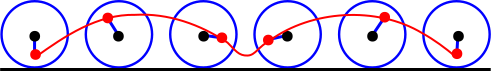
\includegraphics[trim={0 -3mm 0 -3mm}, clip, scale=1]{5_Cycloids3}
%	\end{center}
%
%	There's also the \textbf{prolate cycloid}, formed by a (red) point $P$ on the \textit{exterior} of a given (blue) circle, rolling along the (black) straight line (/axis):
%	
%	\begin{center}
%		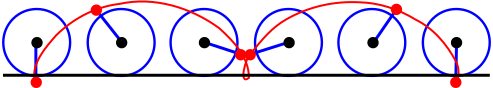
\includegraphics[trim={0 -3mm 0 -3mm}, clip, scale=1]{5_Cycloids4}
%	\end{center}
%
%	\noindent As it happens, the curtate cycloid is defined by parametric equations of the form
%	\begin{equation}
%	\label{eq:cycloids}
%	\left\{
%		\begin{array}{l}
%		x(t)=at-b\sin{t}\\
%		y(t)=a-b\cos{t}
%		\end{array}
%	\right.,\quad0 < t < t_{\text{terminal}}\end{equation}
%	for $a>b$, while the prolate cycloid is defined by the same parametric equations \eqref{eq:cycloids} with $a<b$.
%	
%	\section*{Lima\c{c}ons and Cardioids}
%	Curves defined by parametric equations of the form
%	\begin{equation}
%	\label{eq:limacon}
%	\left\{
%		\begin{array}{l}
%		x(t)=(1+c\sin{t})\cos{t}\\
%		y(t)=(1+c\sin{t})\sin{t}
%		\end{array}
%	\right.,\quad 0 < t < 2\pi\quad(c\text{ constant})\end{equation}
%	are called \textit{lima\c{c}ons}. Figure \ref{fig:limacons} below shows lima\c{c}ons for various values $c$. When $c=\pm 1$, the equations in \eqref{eq:limacon} become
%	\begin{equation}
%	\label{eq:cardioid}
%	\left\{
%		\begin{array}{l}
%		x(t)=(1\pm\sin{t})\cos{t}\\
%		y(t)=(1\pm\sin{t})\sin{t}
%		\end{array}
%	\right.,\quad 0 < t < 2\pi,\end{equation}
%	and the associated curve is called a \textit{cardioid}. Alternatively, ``horizontal analogues'' of \eqref{eq:cardioid} can be obtained by replacing $(1+\sin{t})$ in \eqref{eq:cardioid} by $(1+\cos{t})$:
%	\begin{equation}
%	\label{eq:cardioid2}
%		\left\{
%		\begin{array}{l}
%		x(t)=(1\pm\cos{t})\cos{t}\\
%		y(t)=(1\pm\cos{t})\sin{t}
%		\end{array}
%	\right.,\quad 0 < t < 2\pi.\end{equation}
%	The curves obtained from \eqref{eq:cardioid} and \eqref{eq:cardioid2} are shown in figure \ref{fig:cardioids} below.
%	\begin{figure*}[h!]
%		\centering
%		\begin{subfigure}[t]{0.5\textwidth}
%			\centering
%			\includegraphics[scale=0.5125]{6_Limacons2}
%			\caption{$x(t)=(1\pm\sin{t})\cos{t}$, 
%				$y(t)=(1\pm\sin{t})\sin{t}$\newline(plus in blue, minus in orange)}
%		\end{subfigure}%
%		~ 
%		\begin{subfigure}[t]{0.5\textwidth}
%			\centering
%			\includegraphics[scale=0.5125]{6_Limacons3}
%			\caption{$x(t)=(1\pm\cos{t})\cos{t}$, 
%				$y(t)=(1\pm\sin{t})\cos{t}$\newline(plus in blue, minus in orange)}
%		\end{subfigure}
%		\caption{Vertical and horizontal cardioids}
%		\label{fig:cardioids}
%	\end{figure*}
%
%	\section*{Roses}
%	Consider the parametric curves shown in the following figures:
%	\begin{figure*}[h!]
%		\centering
%		\begin{subfigure}[t]{0.5\textwidth}
%			\centering
%			\includegraphics[scale=0.5125]{7_Roses}
%			\caption{}
%			\label{subfig:roses1}
%		\end{subfigure}%
%		~ 
%		\begin{subfigure}[t]{0.5\textwidth}
%			\centering
%			\includegraphics[scale=0.5125]{7_Roses2}
%			\caption{}
%			\label{subfig:roses2}
%		\end{subfigure}
%		\caption{Various roses.}
%		\label{fig:roses}
%	\end{figure*}
%
%	Unsurprisingly, these curves are called \textit{roses}. There are four general forms for the parametric curves defining roses: The equations defining the roses in figure \eqref{subfig:roses1} have the form
%	\begin{equation}
%		\label{eq:rose}
%		\left\{
%		\begin{array}{l}
%		x(t)=\pm\sin(ct)\cos{t}\\
%		y(t)=\pm\sin(ct)\sin{t}
%		\end{array}
%	\right.,\quad 0 < t < 2\pi\quad(c\text{ constant})\end{equation}
%	(where $+\sin(ct)$ is in blue and $-\sin(ct)$ is in orange), while the equations defining those in \eqref{subfig:roses2} have the form
%	\begin{equation}
%		\label{eq:rose2}
%		\left\{
%		\begin{array}{l}
%		x(t)=\pm\sin(ct)\sin{t}\\
%		y(t)=\pm\sin(ct)\cos{t}
%		\end{array}
%	\right.,\quad 0 < t < 2\pi\quad(c\text{ constant}).\end{equation}
%	(with $+\sin(ct)$ and $-\sin(ct)$ again in blue and orange, respectively).
%	
%	When $c$ is odd, the roses in \eqref{eq:rose} and \eqref{eq:rose2} have $c$ petals; when $c$ is even, they have $2c$ petals. Figure \ref{fig:roses3} below shows curves corresponding to \eqref{eq:rose} for varying values of $c$.
%	
%	In the special case that $c=1$, the result is four ``roses with one petal,'' i.e. circles. In contrast to the circles shown in figure \ref{fig:circle} above, the one-petal roses are tangent to the $x$- and $y$-axes. Figure \ref{fig:roses2} illustrates this case.
%	\begin{figure*}[h!]
%		\centering
%		\begin{subfigure}[t]{0.5\textwidth}
%			\centering
%			\includegraphics[scale=0.5125]{7_Roses4}
%			\caption{$x(t)=\pm\sin{t}\cos{t}$, $y(t)=\pm\sin{t}\sin{t}$\newline(plus in blue, minus in orange)}
%			\label{subfig:roses3}
%		\end{subfigure}%
%		~ 
%		\begin{subfigure}[t]{0.5\textwidth}
%			\centering
%			\includegraphics[scale=0.5125]{7_Roses5}
%			\caption{$x(t)=\pm\sin{t}\sin{t}$, $y(t)=\pm\sin{t}\cos{t}$\newline(plus in blue, minus in orange)}
%			\label{subfig:roses4}
%		\end{subfigure}
%		\caption{Various one-petal roses (i.e., circles tangent to the $x$- and $y$-axes)}
%		\label{fig:roses2}
%	\end{figure*}
%	
%	\section*{Important Note}
%	As we saw in class, replacing $\cos{t}$ and $\sin{t}$ with $\cos(kt)$ and $\sin(kt)$, respectively, in \eqref{eq:circle} will yield a curve which \textbf{graphically} is the same as that rendered by \eqref{eq:circle} but which loops around $k$ times instead of once. 
%	
%	Figure \ref{fig:k} below demonstrates precisely that via the parametric equations $x(t)=\cos(kt)$, $y(t)=\sin(kt)$, $0\leq t\leq 2\pi$, for the values $k=1$, $k=5$, and $k=50$. 
%	
%	Note, too, that for these parametrizations, varying the terminal value $t_{\text{terminal}}$ may also yield the same curve: For example, $x(t)=\cos(kt)$ and $y(t)=\sin(kt)$ yield graphs which are unit circles for all $k$ \textit{and} for all parameter values $0\leq t\leq 2\pi+c$ for all values $c\geq 0$.
%	\begin{figure}[h!]
%		\begin{center}
%			\includegraphics[trim={20mm 0 2mm -6mm}, clip, scale=0.75]{8_Misc}
%			\caption{Curves which are identical as curves but which are \textit{different} as parametric curves (i.e., curves + their associated parametric equations).}
%			\label{fig:k}
%		\end{center}
%	\end{figure}
%	
%	This tells us that parametric curves aren't unique; even more concretely, it tells us that there are often multiple parametrizations which yield the same curve. This fact will be very important when we start doing calculus (e.g., definite integration), because presumably, the mechanisms we employ there should yield correct results while allowing for different parametrizations. These are ideas we'll revisit later.
%	
%	\begin{figure}[h]
%		\begin{center}
%			\includegraphics[trim={20mm 0 3mm 0}, clip, scale=0.825]{4_Spirals3}
%			\caption{The growth of the spiral whose parametric equations are given by $x(t)=t\cos{t}$, $y(t)=t\sin{t}$, for increasing values of $t$.}
%			\label{fig:spirals}
%		\end{center}
%	\end{figure}
%
%	\begin{figure}[h!]
%		\begin{center}
%			\includegraphics[trim={19mm 0 3mm 0}, clip, scale=0.875]{6_Limacons}
%			\caption{Lima\c{c}ons of the form $x(t)=(1+c\sin{t})\cos{t}$, $y(t)=(1+c\sin{t})\sin{t}$ for various values $c$.}
%			\label{fig:limacons}
%		\end{center}
%	\end{figure}
%
%	\begin{figure}[h!]
%		\begin{center}
%			\includegraphics[trim={19mm 0 3mm 0}, clip, scale=0.875]{7_Roses3}
%			\caption{Roses of the form $x(t)=\pm\sin(ct)\cos{t}$, $y(t)=\pm\sin(ct)\sin{t}$, $0<t<2\pi$, for various values of $c$. Note that when $c$ is even, there are $2c$ petals and that the blue and orange curves coincide; otherwise, there are $c$ petals and the blue and orange curves are unique. Also, when $c=0$, $x(t)=0=y(t)$.}
%			\label{fig:roses3}
%		\end{center}
%	\end{figure}
\end{document}